\chapter{Knowledge Under Uncertainty}

In this School of Hard Knocks interview, curated by LazyingArt LLC, the promised Tom Cruise conversation is deliberately delayed. That delay is not empty theater. The lecture uses it to build a sequence of doctrines: first Daniel Lubetzky on brand, distribution, thrift, and structure; then Thomas Healy on scale, pivot, and negotiation; and only then Tom Cruise on passion, fear, and the disciplined conversion of the unknown into applicable knowledge. The chapter therefore reads best not as celebrity summary, but as a study of how large outcomes are assembled under uncertainty.

\section{The Delayed Interview}

The lecture opens with scale before method. Tom Cruise is introduced as one of the greatest movie stars of all time, with decades of visibility, billions at the box office, and hundreds of millions earned personally. But instead of going directly into that promised interview, the narration pivots to Austin and turns the waiting period into a field study of wealth.

That opening move matters. We are not simply being kept away from the headline guest. We are being given intermediate machinery before the final case arrives. The Austin billionaire field is used to answer questions that the Tom Cruise interview alone would not answer cleanly: how a brand is built, how a company should be structured, how one pivots before cash disappears, and how fear can be treated as a knowledge problem rather than merely a temperament problem.

So the order is pedagogically useful:
\begin{equation}
\text{celebrity scale} \;\longrightarrow\; \text{entrepreneurial doctrine} \;\longrightarrow\; \text{craft under risk}.
\end{equation}
The lecture keeps returning to the promised interview, but only after it has accumulated enough comparative material for that interview to land inside a larger theory of success.

\section{Thirty Years Before the Brand}

Daniel Lubetzky enters first, and the lecture immediately resets our scale intuition. Yes, Kind became enormous, but the relevant arithmetic is not just the later annual revenue. It is the length of the build and the number of repetitions that preceded the visible result:
\begin{align}
R_{\mathrm{Kind}} &> \$1\times 10^{9}\ \text{per year},\\
T_{\mathrm{build}} &\approx 30\ \text{years}.
\end{align}
The point is not to worship the later number. It is to recover the long apprenticeship beneath it.

The transcript insists on that apprenticeship. Lubetzky describes roughly ten years of mistakes in natural foods before Kind, an earlier venture connected to conflict regions, family doubt, and an alternative life that could have been spent inside a prestigious legal career. Instead, the lecture gives us the image of the emptied legal suitcase, now filled with products, and the daily rhythm of direct selling. We are told about days beginning around \(7\) a.m.\ and continuing until \(7\) p.m., followed by delivery work and repetition.

That rhythm is better represented by a simple update rule than by a grand theory:
\begin{equation}
N_{t+1}=N_t+\Delta N_t,
\end{equation}
where \(N_t\) is the cumulative number of placements by time \(t\), and \(\Delta N_t\) is one more store, one more shelf, one more successful conversation. The lecture never speaks in this notation, but it does speak in this logic.

If we iterate the rule over many cycles, we obtain the cumulative distribution count
\begin{equation}
N_T = N_0 + \sum_{t=0}^{T-1}\Delta N_t.
\end{equation}
That is the real picture of the Kind story in this lecture. Distribution is not presented as a single retail breakthrough. It is presented as repeated local victories, built slowly enough that later scale looks almost surprising if one ignores the many years underneath it.

\subsection{Question \& Answer}

\paragraph{Question.} What is a brand, and how is it built?

\paragraph{Answer.} The lecture answers this only after the long prehistory has been established. That is important. Brand theory here is not detached marketing language. It is the compression of a long operating history into a few durable rules.

Lubetzky's verbal answer can be summarized in the following light editorial notation:
\begin{equation}
B = \text{value statement} + \text{boundary} + \text{consistency} + \text{promise kept}.
\end{equation}
The first ingredient is positive: what does the brand stand for? The second is negative: what is it not? The lecture is unusually sharp on the necessity of that second part. Without a negative boundary, the brand dissolves into audience-pleasing vagueness.

Consistency is then treated not as mere stubbornness, but as the time variable by which recognition becomes possible. One does not build a mental framework in the customer if colors, logo, tone, and promise are constantly renegotiated. That is why the lecture keeps pressing the same word: consistent, consistent, consistent.

Finally the answer is compressed into one line:
\begin{equation}
\text{great brand} = \text{promise well kept}.
\end{equation}
This is not a theorem. It is a cleaner definition than the usual branding slogans. In the lecture's structure, it arrives only after decades of repetition, which is precisely why it carries weight.

The lecture extends this rule back onto the host's own channel. The point is not self-congratulation. It is a live example of the same mechanism. A viewer returns when he knows what kind of promise is being made and delivered. The chapter should preserve that move because it links consumer brand-building to media brand-building without pretending they are identical businesses.

The lecture then turns from brand identity to money habits. Lubetzky's grandfather supplies the maxim about picking up a penny, and the financial lesson is one of humility rather than glamor. The lecture is not saying that pennies make billionaires through arithmetic alone. It is saying that habits of attention to small units reveal a stance toward effort and waste.

\subsection{Question \& Answer}

\paragraph{Question.} Which entity structure serves growth?

\paragraph{Answer.} Here the lecture stops sounding like branding doctrine and starts sounding like capital-structure doctrine. Lubetzky distinguishes the logic of an LLC from the logic of a C-corp in the context of a business that is profitable and trying to grow.

The transcript's cleanest difference is temporal. In the profitable LLC story, annual success can still generate annual tax consequence at the owner level. In the growth-oriented C-corp story, the emphasis shifts toward retention and reinvestment inside the firm until distribution or liquidity. The core quantity is not simply profit, but retained capital:
\begin{equation}
K_{t+1}=K_t+\Pi_t-D_t,
\end{equation}
where \(K_t\) is retained business capital, \(\Pi_t\) is period profit contribution, and \(D_t\) is distribution to owners.

If we iterate this over many periods, we obtain
\begin{equation}
K_T = K_0 + \sum_{t=0}^{T-1}(\Pi_t-D_t).
\end{equation}
This is the most useful mathematical compression of the segment. If the company is built for growth, then \(D_t\) is kept small, and more capital remains available for reinvestment:
\begin{equation}
D_t \downarrow \qquad \Longrightarrow \qquad K_T \uparrow.
\end{equation}

The lecture's point is not that one legal form is universally superior. It is that growth and extraction imply different time profiles of cash, tax, and compounding. The Busy sponsor block that follows should not be allowed to dominate this section, but the host's recap is still pedagogically useful: structure is not clerical cleanup after the real work is done. It changes what the firm can keep, what it can risk, and how long it can compound internally.

\section{Scale, Pivot, and Negotiation}

Thomas Healy changes the register of the lecture. We move from consumer brand-building into public-company arithmetic, youth at scale, fundraising, and market pivoting. The anchor numbers are part of the teaching:
\begin{align}
a_{\mathrm{Healy,billionaire}} &= 28,\\
V_{\mathrm{Healy},2020} &\approx \$10\times 10^{9},\\
C_{\mathrm{raised}} &\approx \$750\times 10^{6}.
\end{align}
The lecture uses these quantities not only to impress, but to frame a different kind of business environment.

The first environment is the original one: electric trucking and competition with Tesla. The second is the revised one: electric vehicles weaken, competitors are decimated, capital scarcity rises, and the company pivots toward electricity generation, especially for AI data centers, commercial buildings, and industrial applications. The lecture's logic is not hard to formalize:
\begin{equation}
\text{EV downturn} + \text{remaining balance-sheet capital}
\;\longrightarrow\;
\text{pivot into power for AI and industrial demand}.
\end{equation}
This is not generic flexibility. It is a specific relation between market change, preserved internal capital, and the willingness to reassign the firm to a more promising demand surface.

The lecture then asks what separates billionaire-scale operators from merely millionaire-scale ones. Healy's answer is aggressive and simple: winning is the only option. It is not a delicate philosophy, but it matters because it transitions the conversation into the two practical constraints that govern the rest of the segment: avoiding desperation and retaining choice.

\subsection{Question \& Answer}

\paragraph{Question.} How do we fail, and how do we negotiate from strength?

\paragraph{Answer.} The lecture answers the first question by indirection. Companies fail here not because competition exists in the abstract, but because capital runs out before a workable next move exists. That is why the pivot discussion and the negotiation discussion belong together.

The formal compression is
\begin{equation}
L \propto O,
\end{equation}
where \(L\) is negotiation leverage and \(O\) is the number and credibility of outside options. If \(O\) collapses toward zero, desperation rises and leverage falls. If \(O\) is positive and real, one can walk away.

This is exactly what the Florida-investor story is doing in the lecture. A deal is supposed to close. Terms are changed late. Healy does not accept the new terms merely because the clock is advanced. He flies to a different investor and signs the next day. The story is not ornamental. It is a concrete example of leverage as optionality rather than personality.

We may write the underlying contrast as
\begin{equation}
O=0 \;\Longrightarrow\; \text{desperation},
\qquad
O\ge 1 \;\Longrightarrow\; \text{walk-away power}.
\end{equation}
Again, this is editorial notation, but it matches the lecture closely. The segment's final moral is that founders must know their worth and keep a plan B because markets, counterparties, and paths change faster than pride would like to admit.

\section{Passion Is Not Separate From the Work}

Only after two entrepreneurial case studies does the lecture arrive at Tom Cruise. This delay matters because the Cruise segment then sounds less like celebrity mystique and more like a final case in the same larger inquiry: what does large-scale competence look like from the inside?

The first answer is that movies are not one narrow occupation. They encompass almost every industry. Cruise therefore refuses a thin job description. His version of the matter is that this is not merely what he does; it is who he is. That statement must not be smoothed into slogan. In the lecture it is doing real work. It explains why his later remarks about learning, technical detail, crews, and equipment are not distractions from acting, but part of acting rightly understood.

The next conceptual correction is equally important. When the host asks about obsession, Cruise rejects the term and substitutes interest. That move should be preserved carefully. He is not denying intensity. He is refining its tone. ``Obsession'' suggests pathology or narrowing; ``interest'' suggests active, delighted, disciplined curiosity. The lecture wants us to see excellence not as fever, but as sustained involvement with many layers of reality.

That is why the section moves naturally from identity to risk. Once the work is understood as total involvement rather than surface performance, fear can no longer be treated as mere attitude. It has to be explained as a relation between the person and the unknown features of the task.

\section{Knowledge Against the Unknown}

This is the deepest section of the lecture. Cruise is asked about fear and risk, and he gives an answer that is almost algorithmic in its structure. He does not claim to feel nothing. He says he does not mind being afraid, because fear is the unknown. That is the key sentence.

The lightest faithful formalization is
\begin{equation}
A\uparrow \;\Longrightarrow\; U\downarrow \;\Longrightarrow\; F\downarrow,
\end{equation}
where \(A\) is applicable knowledge, \(U\) the unknown, and \(F\) fear. The lecture's point is not that all adrenaline disappears. It is that fear ceases to govern once the unknown is turned into something studied, tested, and embodied.

Cruise then describes how this works in practice. One begins with a shot or goal, and then one builds the chain of knowledge required to produce correct results:
\begin{equation}
G \longrightarrow \mathcal{K}(G) \longrightarrow \mathcal{T}(G) \longrightarrow R_{\mathrm{correct}}.
\end{equation}
Here \(G\) is the goal, \(\mathcal{K}(G)\) the list of things that must be known, \(\mathcal{T}(G)\) the associated training and preparation program, and \(R_{\mathrm{correct}}\) the reliable outcome.

The lecture gives the contents of \(\mathcal{K}(G)\) in concrete terms. If the shot involves hanging off an aircraft, then one must understand not only performance, but aircraft maneuvers, the pilot's knowledge, stall conditions, wind and fuel behavior over the wing, camera equipment, specially developed technology, bodily movement, and the training needed to survive the forces involved. The actor is not simply ``doing a stunt.'' He is entering a system of interacting constraints and making each of them less mysterious.

\begin{figure}[h]
\centering
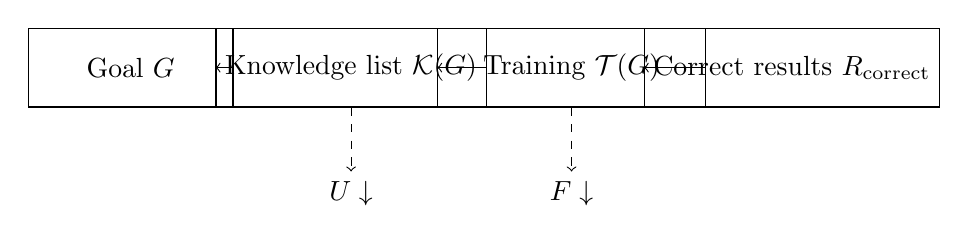
\begin{tikzpicture}[node distance=2.8cm, auto]
\node[draw, rectangle, minimum width=2.6cm, minimum height=1cm] (goal) {Goal \(G\)};
\node[draw, rectangle, right of=goal, minimum width=3.2cm, minimum height=1cm] (knowledge) {Knowledge list \(\mathcal{K}(G)\)};
\node[draw, rectangle, right of=knowledge, minimum width=3.4cm, minimum height=1cm] (training) {Training \(\mathcal{T}(G)\)};
\node[draw, rectangle, right of=training, minimum width=2.9cm, minimum height=1cm] (results) {Correct results \(R_{\mathrm{correct}}\)};

\draw[->] (goal) -- (knowledge);
\draw[->] (knowledge) -- (training);
\draw[->] (training) -- (results);

\node[below of=knowledge, node distance=1.6cm] (unknown) {\(U\downarrow\)};
\node[below of=training, node distance=1.6cm] (fear) {\(F\downarrow\)};

\draw[dashed, ->] (knowledge) -- (unknown);
\draw[dashed, ->] (training) -- (fear);
\end{tikzpicture}
\caption{Transcript-derived schematic of the lecture's planning loop: the unknown is reduced by converting a goal into a knowledge program and then into training, equipment, and collaboration.}
\end{figure}

\subsection{Question \& Answer}

\paragraph{Question.} How does knowledge reduce fear?

\paragraph{Answer.} Not by argument alone, and not by pretending the dangerous thing is harmless. The lecture's answer is that one must know and experience enough of the problem that the unknown ceases to dominate. Cruise is explicit that if something is not true for him, it is not true for him. He has to experience and understand it for himself.

That is why the lecture rejects the fantasy that one can simply sit in a room, sketch the shot, and thereby possess it. There is always a physical question: how do we train to get here? There is always a technical question: what equipment must exist for the image to be captured? There is always a collaborative question: what must the pilot know, what must the director know, what must the whole film group align on?

We can therefore rewrite the fear problem more concretely as
\begin{equation}
U = U_{\mathrm{technical}} + U_{\mathrm{physical}} + U_{\mathrm{collaborative}},
\end{equation}
and the lecture's method is to reduce each term by learning, rehearsal, equipment design, and repeated testing. No such equation is spoken, but the decomposition is faithful to the structure of the answer.

The same logic explains why Cruise prefers ``interest'' to ``obsession.'' Interest is the durable stance that keeps asking what still remains unknown. Fear diminishes not when we become numb, but when we become more competent.

Cruise then extends this into work ethic. Excellence interests him, he says, while absolutes remain unattainable. The right mathematical picture is therefore not possession, but asymptotic striving. We keep moving toward a standard that cannot be finally owned, and we do so because we want to deliver the best work we can.

\section{Summary}

The lecture begins as a promise to interview Tom Cruise and ends as a broader theory of applied knowledge under uncertainty. Lubetzky teaches that a brand is built by long repetition, clear boundaries, and a promise well kept. Healy teaches that scale survives only when capital is preserved long enough to pivot and when negotiation is backed by real options. Cruise teaches that fear is the unknown, and that the way through it is not bravado but the organized acquisition of knowledge that can be applied.

If we compress the whole chapter into one line, it is this: the visible result is never the whole story. Under the result sits repetition, retained capital, credible alternatives, and the conversion of uncertainty into disciplined understanding. That is the lecture's most durable lesson, and it is what allows celebrity, entrepreneurship, and craft to live inside one argument without collapsing into spectacle.